%
% $ID$
%
% $Log$
% Revision 1.4  2005/10/27 16:46:29  sliver
% *** empty log message ***
%
% Revision 1.3  2005/10/26 15:40:51  sliver
% *** empty log message ***
%
% Revision 1.2  2005/10/26 14:34:50  sbecker
% Added section on method based design by contract and type systems
%
%

\section{Foundations} % Arbeitstitel!
\label{sec:foundations}

The Palladio component meta modell mainly bases on concepts for
components presented by the OMG in the UML 2.0 standard and parametric contracts
that model the intra-component dependencies of provided and required interfaces.
Both concepts are introduced in the following. 

\subsection{UML 2.0 Component Concepts}

An \emph{assembly connector} connects a required interface of an inner component
to a provided interface
of another inner component. 

\emph{Delegation connectors} map provided and required
interfaces of the composite component to interfaces of its inner
structure. 

A provides delegation connector maps
a provided interface of the composite component to provided interface of an
inner component. 

A requires delegation connector maps a required interface of an
inner component to a required interface of the composite component.

\subsection{Types and Design-by-Contract}
\label{types_design_by_contract}

A central idea of a type system is to allow \emph{subtyping}. The basic idea is that a subtype of a given supertype can be used at every place where an instance of the supertype was expected. Taking design-by-contract \cite{meyer1997a} \footnote{A formal definition can be found in the book by Meyer \cite{meyer1997a}} into consideration this has several implications:

\begin{itemize}
\item The precondition of every operation of the type has to be weaker than the supertype's operation precondition.
\item The postcondition of every operation of the type has to be stronger than the supertype's operation postcondition.
\item Any invariant of the supertype has also to be true for all subtypes.
\end{itemize}

Note that every type which is used in any kind of declaration is already a contract stating that the values contained in the declared variable conform to the specified type. Hence, the rules given above can be applied to type declarations as well. Applying this to the parameter and the return types of an arbitrary operation being part of an inheritance hierarchy leads to a type system which is contra-variant. A discussion on the advantages and disadvantages of so doing can be found in \cite[p. 628ff]{meyer1997a}.

Another use of a type system is to perform conformance checks. Conformance checks are useful if one has to decide whether a certain communication between a client and a server is contractually safe, i.e., does not result in a run-time error. For this, a necessary condition is that the required interface has to be a supertype of the provided interface it is bound to. 

\subsection{Parametric Contracts}

Component contracts lift the Design-by-Contract principle of Meyer (``if a
client fulfils the precondition of a supplier, the supplier guarantees the
postcondition'' \cite{meyer1992a}) from methods to software components. A
component guarantees to offer the functionality specified by its provided
interfaces (postcondition) if all required interfaces are offered by its
environment. Design-by-Contract cannot only be applied to
functional properties, but also to non-functional properties. Adding Quality of
Service (QoS) attributes to the contract, a component ensures that it
provides a certain QoS if its environment offers the required QoS attributes. 

Parametric contracts \cite{reussner2002c} extend the design by contract
principle of software components. The provided interfaces (postcondition) of a
component are computed in dependence on the actual interfaces offered by the
environment (precondition). The relationship between provided and required
interfaces of a software component can be used to compute the influence of
external services used by the component on its QoS attributes as well. We
distinguish between \emph{basic components} and \emph{composite components} as
two different ways of implementing a component.

We state that a component can still be considered a black-box entity if the
additional information used by parametric contracts (a) does not expose
intellectual property of the component vendor and (b) has not to be understood
by human users. So, the additional information and its analysis has to be
transparent for the deployer.

A \emph{service effect specification} describes the relationship between
provided and required interfaces. It defines the externally visible behaviour of
a provided service. This includes the used external services, possible call
sequences, and, for example, probabilities of service calls. A service effect
specification can be modelled in different ways. It can be a signature list that
only contains the called external services. It can model all possible call
sequences executed by a provided service. This can be expressed by different
means, for example, finite state machines, Petri nets, regular expressions, or
any other kind of grammar. In any case, a service effect specification is an
abstraction of component source code. It models calls to external services only
and neglects the internal component code.

\begin{figure}[htbp]
\centering
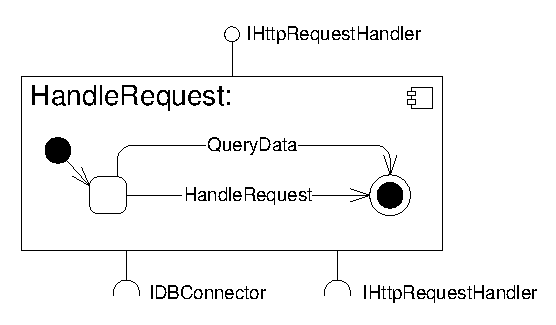
\includegraphics[scale=0.85]{example/HandleRequestSEFF}
\caption{Service effect specification of the method HandleRequest in the
DynamicFileProvider.}
\label{fig:seff}
\end{figure}

Figure \ref{fig:seff} shows a simple service effect specification modelled as a
finite state machine. If the method HandleRequest of the DynamicFileProvider is
responsible for the incoming request it executes a query on the connected
database. In the internal code that is not visible here, it creates the web page
and returns the result to the client. If it is not responsible for the incoming
request it forwards the request to the next component in the chain of
responsibility. This is done by the call of the HandleRequest method of the
component connected to the IHttpRequestHandler interface.

Discuss what is modelled by a service effect specification. What is an external
service?
